\documentclass[10pt,twocolumn,a4paper]{article}

\usepackage[T1]{fontenc}
\usepackage[utf8]{inputenc}
\usepackage{lmodern}
\usepackage{microtype}
\usepackage[a4paper,top=1.55cm,bottom=1.7cm,left=1.6cm,right=1.6cm,columnsep=0.55cm]{geometry}
\usepackage{amsmath,amssymb}
\usepackage{graphicx}
\usepackage{booktabs}
\usepackage{array}
\usepackage[font=small,labelfont=bf,justification=raggedright,singlelinecheck=false,skip=3pt]{caption}
\usepackage{titlesec}
\usepackage{enumitem}
\usepackage{xcolor}
\usepackage{fancyhdr}
\usepackage{needspace}
\usepackage{balance}
\usepackage[pdftitle={RUIN: Seeing When Physical Systems Run Out of Destiny},pdfauthor={Naji Zouiti},pdfsubject={Ruin probability and remaining destiny for logistics},colorlinks=true,linkcolor=blue!45!black,citecolor=blue!45!black,urlcolor=blue!45!black]{hyperref}

\titleformat{\section}{\normalfont\large\bfseries\scshape}{\thesection}{0.6em}{}
\titlespacing*{\section}{0pt}{1.0ex plus 0.3ex minus 0.2ex}{0.4ex plus 0.1ex}
\titleformat{\paragraph}[runin]{\normalfont\normalsize\bfseries}{}{0pt}{}
\titlespacing*{\paragraph}{0pt}{0.5ex plus 0.2ex}{0.6em}

\setlength{\parindent}{1em}
\setlength{\parskip}{0pt}
\setlength{\abovedisplayskip}{3pt plus 1pt minus 2pt}
\setlength{\belowdisplayskip}{3pt plus 1pt minus 2pt}
\setlength{\abovedisplayshortskip}{2pt}
\setlength{\belowdisplayshortskip}{2pt}
\setlength{\textfloatsep}{7pt plus 2pt minus 2pt}
\setlength{\floatsep}{6pt plus 2pt minus 2pt}
\setlength{\intextsep}{6pt plus 2pt minus 2pt}
\widowpenalty=10000
\clubpenalty=10000
\raggedbottom

\pagestyle{fancy}
\fancyhf{}
\renewcommand{\headrulewidth}{0pt}
\fancyfoot[C]{\small\thepage}
\fancyhead[L]{\small\itshape RUIN: seeing when physical systems run out of destiny}
\fancypagestyle{plain}{\fancyhf{}\renewcommand{\headrulewidth}{0pt}\fancyfoot[C]{\small\thepage}}

\newcommand{\ruin}{\textsc{Ruin}}

\makeatletter
\renewcommand{\maketitle}{%
  \begin{center}
    {\LARGE\bfseries RUIN: Seeing When Physical Systems\\[2pt] Run Out of Destiny\par}
    \vspace{5pt}
    {\large Naji Zouiti\par}
    \vspace{2pt}
    {\small Software version 0.9.1\ \ $\cdot$\ \ November 2026\ \ $\cdot$\ \ \url{github.com/nezpik/ruin}\par}
  \end{center}}
\makeatother

\begin{document}

\twocolumn[%
\maketitle
\begin{center}
\begin{minipage}{0.88\textwidth}
\small
\textbf{Abstract.}\ Logistics rarely fails on an average day; it fails on a bad one. Averages hide bad days, while insurance mathematics has a mature theory of \emph{ruin}, the moment a reserve runs out, for exactly this kind of event. \ruin{} carries that theory from money to physical flow. Deliveries travel across a bounded grid shaken by a spreading disruption field whose intensity is driven by a hidden regime; a shift is ruined when its buffer is spent or its service promise is broken. \ruin{} estimates the probability of ruin, the size of the tail loss and \emph{remaining destiny}: the chance a shift still has of finishing safely given what is known now. We check it against exact ruin theory, test it against eight qualitative regularities of disruption, and show that in our reference scenario, at the same average disruption, a steady world never ruins while a bursty one ruins about one shift in six. \ruin{} is an abstract research instrument, not a calibrated forecaster.

\smallskip
\textbf{Keywords:} logistics, ruin theory, disruption, regime switching, resilience, simulation.
\end{minipage}
\end{center}
\vspace{4pt}
]

\section{Why ruin?}
Logistics rarely fails on an average day. It fails on a bad one: a storm, an accident and a failed hand-off arrive together, queues feed on themselves, and an operation that looked comfortable on paper can no longer keep its promises or cover its costs. We call that moment \emph{ruin}. Most planning tools describe average delay or average load, and averages hide exactly these days.

Insurance mathematics has asked the same question for a century \cite{cramer1930,asmussen2010}: given steady income and random claims, how likely is it that a reserve is ever exhausted, and when? \ruin{} carries the question from money to physical flow. That is not a small change. Disruptions in a physical system are not independent claims: they land in particular places, spread to neighbouring ones, linger where traffic is stuck, and are made worse by the system's own congestion. Traffic-flow and network-cascade models study related mechanisms \cite{daganzo1994,buldyrev2010}; \ruin's object is different, namely whether a \emph{service} survives.

\ruin{} is a \emph{research instrument}, not a forecasting product. It is for (i) asking how an operation fails and not only how often, (ii) comparing scenarios and, later, protective policies, (iii) teaching and building intuition, and (iv) turning a vague word, resilience, into quantities that can be measured and argued over. It is deliberately abstract: there are no maps and no customer data yet, so every number below describes a stylised scenario. Read it as a property of the model, not as a prediction about a real operation.

\section{The idea in plain words}
A shift of work plays out inside the \emph{destiny frame} $D$, a bounded grid: the stage on which every possible future of the shift unfolds, and from which nothing can escape. Five ingredients populate it.
\begin{description}[leftmargin=0pt,labelsep=0.4em,itemsep=1pt,parsep=0pt,topsep=2pt]
\item[Q dots] are deliveries, quantised attempts at order. Each has an origin, a destination and a time window. Arriving in time earns income; each step of lateness costs a penalty.
\item[Disruption] arrives as shocks that land at random places, spread to neighbours and fade. Where it is strong a cell is blocked and Q dots crawl. A connected blocked region is a \emph{jam}.
\item[A hidden regime] says what $D$ is doing: stable, stressed, disrupted or chaotic. It sets how often and how large shocks are. Regimes last (a bad day stays bad), change one level at a time, are pushed toward worse levels by the system's own lateness and eased by healthy flow. Nobody sees the regime directly; an operator sees only pressures.
\item[Surplus] is the buffer: a starting reserve, plus income, minus penalties.
\item[Ruin] has two doors: the surplus is spent, or the service promise is broken because too many deadlines are missed.
\end{description}
Running thousands of simulated shifts (a \emph{Monte Carlo} study) turns this into probabilities. Figure~\ref{fig:anatomy} follows one shift.

\begin{figure*}[t]
\centering
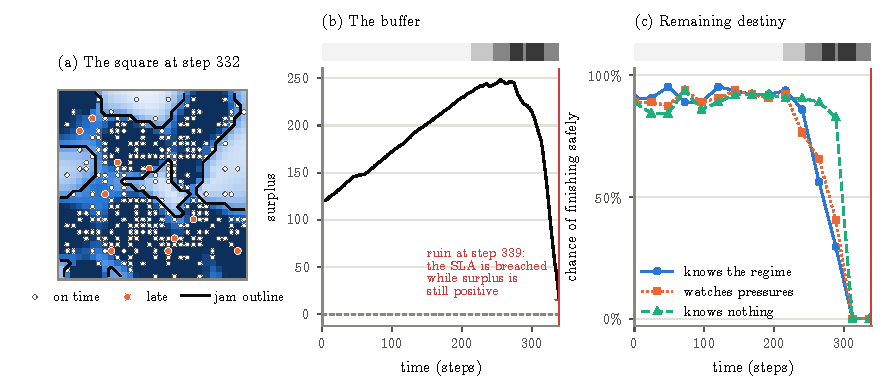
\includegraphics[width=\textwidth]{figures/anatomy.pdf}
\caption{One simulated shift (reference scenario, seed 81). \textbf{(a)}~At step 332 a single jam (outlined) covers 75\% of the square; darker blue means more disruption, orange dots are late deliveries. \textbf{(b)}~The buffer climbs to 248 by step 255, just as the regime turns disrupted (step 245), and the shift is ruined at step 339 by a breached promise while the surplus is still 14. \textbf{(c)}~Chance of finishing safely, from 64 simulated futures at each checkpoint, for an observer who knows the hidden regime (solid), one who sees pressures and incident reports (dotted) and one who knows nothing about it (dashed). The grey bars above (b) and (c) show the hidden regime; darker is worse.}
\label{fig:anatomy}
\end{figure*}

\section{The mathematics in brief}
Seven short formulas carry the model; each has a plain reading.

\paragraph{Buffer and ruin.} The surplus is
\begin{equation}\label{eq:surplus}
U(t)=U(0)+C(t)-L(t),
\end{equation}
the starting reserve plus recovery and on-time income $C(t)$, minus the lateness penalties $L(t)$ paid so far. Ruin is the first time at which either door opens:
\begin{align}
\tau&=\min\{t:\ U(t)\le b\ \ \text{or}\ \ m_w(t)\ge s\},\label{eq:ruin}\\
m_w(t)&=\frac{\text{missed}}{\text{missed}+\text{on time}}\ \text{over the last } w \text{ steps},\notag
\end{align}
where $b$ is the barrier and $s$ the promised limit on the share of missed deadlines.

\paragraph{Disruption cannot feed itself.} Let $x_t$ be the disruption in every cell. Then
\begin{equation}\label{eq:field}
x_{t+1}=g\big[(1-\sigma)I+\sigma K\big]x_t+\xi_t,\qquad g<1:
\end{equation}
each step a cell keeps a fraction $g$ of its disruption, a share $\sigma$ of what it keeps moves to neighbours ($K$), and new shocks $\xi_t$ arrive. Because $g<1$ the total grows only when shocks arrive. Where Q dots are stuck $g$ rises toward a cap that is still below one, so jams linger but cannot grow by themselves.

\paragraph{The hidden regime.} From level $k$ (0 stable, 3 chaotic) the chance of moving up or down in one step is
\begin{align}
P(k\!\to\!k{+}1)&=e_k\,\phi\,(1-\kappa\,o_t),\notag\\
P(k\!\to\!k{-}1)&=r_{k-1}\,\phi\,(1+\kappa\,o_t),\label{eq:regime}
\end{align}
with base rates $e_k,r_k$; $o_t$ the share of deliveries that are flowing (order pressure); and $\phi=p$ if the move heads toward the level that the system's chaos pressure points to, $1/p$ if it heads away, and $1$ otherwise. Late deliveries raise pressure, pressure pulls the regime up and healthy flow resists: deliveries and $D$ co-evolve.

\paragraph{Remaining destiny.} The central quantity is
\begin{align}
\Delta(t)&=\Pr\!\big(\text{no ruin before } T\mid\text{state at } t\big)\label{eq:destiny}\\
&\approx\frac1N\sum_{i=1}^{N}\mathbf 1\{\text{future } i\ \text{survives}\}.\notag
\end{align}
It is estimated by freezing the exact present and playing out $N$ independent futures. It starts near one minus the ruin probability and falls to zero at ruin: a shift \emph{runs out of destiny} when $\Delta$ reaches zero.

\paragraph{What an observer can know.} An operator sees pressures, not the regime. The belief $b_t(k)$ that $D$ is in regime $k$ follows Bayes' rule:
\begin{equation}\label{eq:filter}
b_t(k)\ \propto\ \Big[\sum_{j}b_{t-1}(j)\,T_{jk}\Big]\,\ell_t(k)^{\theta}.
\end{equation}
It predicts through the known chain $T$ (Eq.~\ref{eq:regime}, which depends only on pressures the observer sees), then weights by how likely the readings $\ell_t(k)$ are under each regime. The exponent $\theta=0.4$ tempers the evidence, because successive readings are not independent.

\paragraph{A benchmark with a known answer.} Remove space and regimes, and feed Eq.~\eqref{eq:surplus} a constant premium rate $c$ and random claims (rate $\lambda$, mean size $\mu$). The ruin probability for initial reserve $u$ is then known exactly \cite{asmussen2010}:
\begin{equation}\label{eq:cl}
\psi(u)=\frac{\lambda\mu}{c}\,\exp\!\Big[-\Big(\frac1\mu-\frac\lambda c\Big)u\Big].
\end{equation}
The simulator's accounting of ruin must reproduce it, and it does (Table~\ref{tab:cl}).

\section{What \ruin{} adds}
\paragraph{A shared, measurable language.} Table~\ref{tab:translate} maps insurance and finance onto logistics. The mapping is not a metaphor: each row is an object in the code with a number attached, so ``resilience'' becomes a ruin probability, a tail loss and a remaining destiny.

\begin{table}[t]
\centering\small
\caption{From insurance and finance to logistics. Hedging is future work.}
\label{tab:translate}
\renewcommand{\arraystretch}{1.08}
\begin{tabular}{@{}ll@{}}
\toprule
Finance and insurance & In \ruin \\
\midrule
Reserve & Operating buffer (surplus) \\
Claims & Disruptions: storms, accidents \\
Ruin & Buffer spent or promise broken \\
Tail risk \cite{mcneil2015,rockafellar2000} & Tail loss over a shift \\
Regime switching \cite{hamilton1989} & Stable to chaotic days \\
Hedging & Buffers, backup, rerouting \\
\bottomrule
\end{tabular}
\end{table}

\paragraph{Remaining destiny as a gauge.} Surplus alone is a poor warning light. In Figure~\ref{fig:anatomy} the surplus stood near its maximum when the crisis began, while the buffer the shift would have needed for a 95\% chance of safety jumped from about 250 (step 216) to over 1,100 (step 264). Remaining destiny sees the crisis building; the surplus does not.

\paragraph{Structure beats averages.} At the same average disruption, whether disruption arrives steadily or in bursts decides whether an operation is safe (Section~\ref{sec:found}). A model that knows only averages cannot see this. \ruin{} makes the structure of disruption an explicit, testable assumption.

\paragraph{Validation by design.} A simulator without data cannot be calibrated, but it can be checked: against exact theory (Eq.~\ref{eq:cl}), against eight qualitative regularities that a memoryless model mostly fails, with intervals on every headline number, and with a stated limit for each result. Ruin probabilities are reported as properties of a structure, not as facts about the world.

\paragraph{Seeing what cannot be seen.} The hidden regime and the observer turn a worry, ``we cannot see the crisis coming'', into a quantity: how much of the value of knowing the regime can be had by watching.

\section{What we found}\label{sec:found}
\paragraph{It reproduces theory.} Table~\ref{tab:cl} compares exact ruin probabilities with the simulator on 20,000 paths each; every exact value lies inside the 99\% interval.

\begin{table}[t]
\centering\small
\caption{Simulated against exact ruin probability (Eq.~\ref{eq:cl}; $\lambda{=}1$, $\mu{=}1$, $c{=}1.5$).}
\label{tab:cl}
\begin{tabular}{@{}cccc@{}}
\toprule
Reserve $u$ & Exact & Simulated & 99\% interval \\
\midrule
0 & 0.6667 & 0.6699 & 0.661--0.678 \\
2 & 0.3423 & 0.3400 & 0.331--0.349 \\
5 & 0.1259 & 0.1236 & 0.118--0.130 \\
10 & 0.0238 & 0.0231 & 0.021--0.026 \\
\bottomrule
\end{tabular}
\end{table}

\paragraph{It shows the regularities we test for.} These are qualitative features that disruption is commonly reported to have; we have not checked them against data. The reference scenario shows all eight: disruption clusters in time, bad stretches persist, shift losses and trip times have heavy tails, service varies between good and bad days, clustered disruption costs more than steady disruption of the same mean, the regime is only partly observable, and pressure pushes the regime. The memoryless version of the same scenario shows one of the six that apply to it.

\paragraph{Averages hide bad days.} Figure~\ref{fig:structure} runs the scenario under four structures of disruption with the same measured mean (148 units of shock mass per step). Steady disruption never ruined a shift (0 of 400; 95\% interval 0--0.9\%), heavy-tailed sizes alone changed nothing, but bursts alone ruin 11.8\% of shifts and the full scenario 15.5\%. Ruin here is a property of crises, not of the average level of disruption.

\begin{figure}[t]
\centering
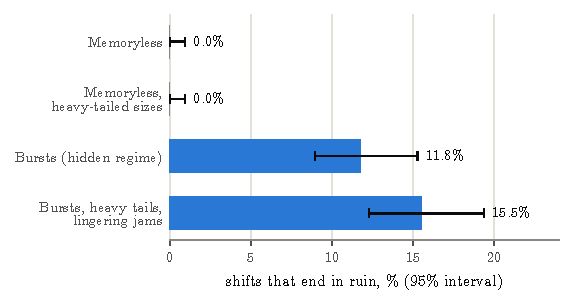
\includegraphics[width=\columnwidth]{figures/structure.pdf}
\caption{Same average disruption, very different ruin (400 shifts each).}
\label{fig:structure}
\end{figure}

\paragraph{Ruin is one gridlock.} Jams (Fig.~\ref{fig:org}) form about every three steps, live nine steps, occupy 11\% of cell-steps and carry 53\% of the loss. The regime does not change typical jams; it fattens the tail. In the ruined shifts, the jam that took the shift averaged 486 cells (54\% of the grid), carried 57\% of the loss in the 24 steps before ruin and was born in a disrupted or chaotic regime in six of seven. Cause and effect are also separated in time (Fig.~\ref{fig:cause}): the disrupted and chaotic regimes are 9\% of the time, 22\% of the delay and 49\% of the loss, because lateness compounds.

\begin{figure}[t]
\centering
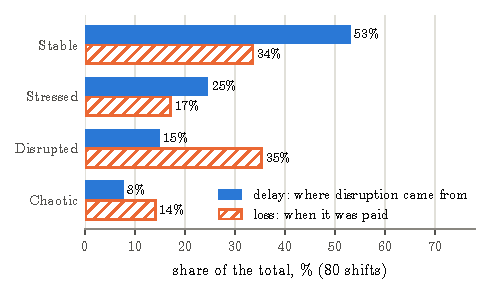
\includegraphics[width=\columnwidth]{figures/cause_effect.pdf}
\caption{Where the delay came from, against when the loss was paid.}
\label{fig:cause}
\end{figure}

\begin{figure*}[t]
\centering
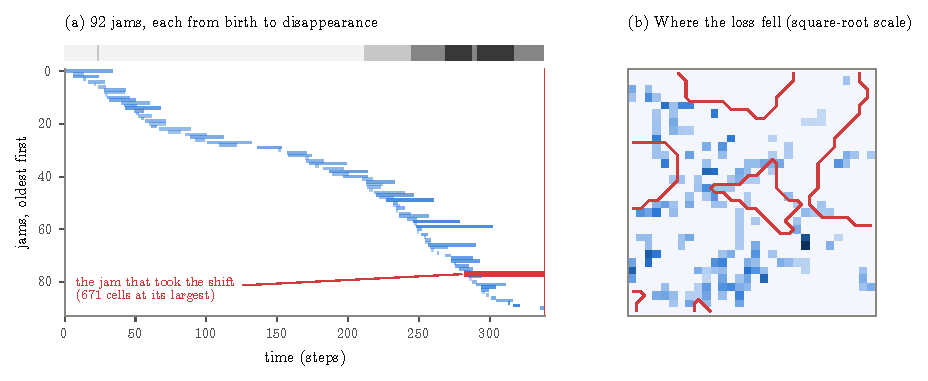
\includegraphics[width=\textwidth]{figures/organization.pdf}
\caption{The organisation of the shift in Figure~\ref{fig:anatomy}. \textbf{(a)}~Each bar is one jam, from birth to disappearance (darker is larger at its peak); the grey bar above shows the hidden regime. Small jams come and go all shift; the one outlined in red, which spans most of the square at its largest, takes the shift. \textbf{(b)}~Where loss fell, with that jam's largest extent outlined.}
\label{fig:org}
\end{figure*}

\paragraph{Watching recovers a third of what knowing would.} On 80 held-out shifts the observer scores a log score of $-0.54$ against $-0.75$ for knowing nothing, and is close to calibrated. Over 32 unselected shifts, in severe regimes it closes 31\% (95\% interval 14--43\%) of the gap between knowing nothing about the regime and knowing it; Figure~\ref{fig:anatomy}(c) is a crisis chosen to show the effect, and a typical shift shows less. With only six ruined shifts the observer cannot be separated from knowing nothing when scored against what actually happened.

\paragraph{Steering helps, but opens no routes.} Letting Q dots steer around blocked cells cuts mean loss by 43\% and ruin from 15.5\% to 9.5\% at the strongest setting. It does so by keeping dots out of jams, not by opening corridors: with monotone trips a dot can choose between its two forward moves but cannot detour.

\section{Where it stands, and where it goes}
\paragraph{Present.} \ruin{} 0.9.1 is open-source Python (MIT licence) of about 5,600 lines with 255 automated tests, seeded and reproducible runs, and commands to simulate, estimate risk, follow remaining destiny, fit an observer, measure structure, and test the model against its regularities and against exact theory.

\begin{table}[t]
\centering\small
\caption{What is in the box: each command and the question it answers.}
\label{tab:box}
\renewcommand{\arraystretch}{1.1}
\begin{tabular}{@{}>{\ttfamily\footnotesize}p{0.2\columnwidth}>{\raggedright\arraybackslash}p{0.74\columnwidth}@{}}
\toprule
\normalfont Command & \normalfont The question \\
\midrule
risk & How often does a shift end in ruin, and how bad is the tail? \\
destiny & How much destiny does this shift have left, right now? \\
structure & Does the answer depend on the shape of disruption? \\
observer & How much of the hidden regime can an operator see? \\
organize & How does disruption organise, and which jam causes ruin? \\
facts, validate & Does the model behave like disruption, and match exact theory? \\
sensitivity, uncertainty & Which assumptions move the answer most? \\
simulate & What does one shift look like? \\
\bottomrule
\end{tabular}
\end{table}

\paragraph{Limits.} The grid is abstract and the parameters are illustrative, never fitted to data. Shocks land uniformly and trips are monotone, so corridors and persistent hot spots cannot form. The observer is fitted with the true regime labels, which a real operator never has, so a real one should do somewhat worse. Steering assumes perfect local information at no cost. All results come from one reference scenario.

\Needspace{7\baselineskip}
\paragraph{Future work.}
\begin{enumerate}[leftmargin=1.4em,itemsep=1pt,parsep=0pt,topsep=2pt,label=\arabic*.]
\item A \emph{policy layer}: buffers, backup capacity and rerouting ranked by ruin averted per unit cost, evaluated through the observer and across structures of disruption.
\item \emph{Real topology}: road graphs and depots, where corridors and persistent hot spots can exist.
\item \emph{Calibration}: fitting the regime chain to operational data, a natural hidden-Markov problem.
\item Deadlines that depend on trip length, and congestion that slows travel.
\item A head-to-head comparison with conventional simulation tools, and studies with practitioners of whether destiny curves change decisions.
\end{enumerate}

\balance
\begin{thebibliography}{9}\small
\setlength{\itemsep}{0pt}\setlength{\parsep}{0pt}
\bibitem{cramer1930} H.~Cram\'er. On the mathematical theory of risk. \emph{Skandia Jubilee Volume}, Stockholm, 1930.
\bibitem{asmussen2010} S.~Asmussen and H.~Albrecher. \emph{Ruin Probabilities}, 2nd ed. World Scientific, 2010.
\bibitem{daganzo1994} C.~F. Daganzo. The cell transmission model. \emph{Transportation Research B} 28(4):269--287, 1994.
\bibitem{buldyrev2010} S.~V. Buldyrev et al. Catastrophic cascade of failures in interdependent networks. \emph{Nature} 464:1025--1028, 2010.
\bibitem{mcneil2015} A.~J. McNeil, R.~Frey and P.~Embrechts. \emph{Quantitative Risk Management}, rev. ed. Princeton University Press, 2015.
\bibitem{rockafellar2000} R.~T. Rockafellar and S.~Uryasev. Optimization of conditional value-at-risk. \emph{J. Risk} 2(3):21--41, 2000.
\bibitem{hamilton1989} J.~D. Hamilton. A new approach to the economic analysis of nonstationary time series and the business cycle. \emph{Econometrica} 57(2):357--384, 1989.
\end{thebibliography}

\end{document}
